%%%%%%%%%%%%%%%%%%%%%%%%%%%%%%%%%%%%%%%%%%%%%%%%%%%%%%%%%%%%%%%%%%%%%%
% 
% 	Template for Producing ASP-DAC 2018 Proceedings
% 
%%%%%%%%%%%%%%%%%%%%%%%%%%%%%%%%%%%%%%%%%%%%%%%%%%%%%%%%%%%%%%%%%%%%%%
% History
% ??/??/?? Designed by Hiroaki Kunieda (ASP-DAC '97 Publication Chair)
% 09/22/97 Modified and small bug fixed by Masaharu Imai 
% 	   (ASP-DAC '98 Publication Chair)
% 11/02/98 Modified by Tsuyoshi Isshiki
% 	   (ASP-DAC 2000 TPS Secretary)
% 7/24/00 Modified by Kiyoharu Hamaguchi
% 	   (ASP-DAC 2001 Publication chair)
% 6/18/02 Modified by Kazutoshi Kobayashi
% 	   (ASP-DAC 2003 Publication Co-Chair)
% 5/27/03 Modified by Kiyoharu Hamaguchi
% 	   (ASP-DAC 2004 TPC secretary)
% 6/10/03 Modified by Kazutoshi Kobayashi for Latex2e
% 	   (ASP-DAC 2004 Publication Co-Chair)
% 6/01/05 Modified by Nozomu Togawa
% 	   (ASP-DAC 2006 Publication Chair)
% 6/01/06 Modified by Hiroyuki Ochi
% 	   (ASP-DAC 2007 Publication Chair)
% 5/30/08 Modified by Nozomu Togawa
% 	   (ASP-DAC 2009 Publication Co-Chair)
% 4/30/10 Modified by Masashi Imai
% 	   (ASP-DAC 2011 Publication Chair)
% 3/20/12 Modified by Masashi Imai
% 	   (ASP-DAC 2013 Publication Chair)
% 5/01/14 Modified by Masashi Imai
% 	   (ASP-DAC 2015 Publication Chair)
% 4/24/16 Modified by Masashi Imai
% 	   (ASP-DAC 2017 Publication Chair)
% 2/06/17 Modified by Jongeun Lee
% 	   (ASP-DAC 2018 Publication Chair)
%%%%%%%%%%%%%%%%%%%%%%%%%%%%%%%%%%%%%%%%%%%%%%%%%%%%%%%%%%%%%%%%%%%%%%
% If you have any problem, please contact ASP-DAC 2018 Publication
% Chair by E-mail at "jlee@unist.ac.kr.''
%%%%%%%%%%%%%%%%%%%%%%%%%%%%%%%%%%%%%%%%%%%%%%%%%%%%%%%%%%%%%%%%%%%%%%
%
\documentclass[twocolumn]{article}
%% If you use dvips and ps2pdf, please use Postscript font 
%% and uncomment the line below.
%%\usepackage{times}
\usepackage[dvipdfmx]{graphicx}
\pagestyle{empty}
%set paper size
%for A4 paper
\topmargin      29mm    %bottom margin 30mm
\oddsidemargin  15mm    %left & right margin 15mm

%for 8 1/2" x 11" paper paper, use the following definition
%\topmargin     17mm    %bottom margin 24mm
%\oddsidemargin 18mm    %left margin 18mm & right margin 17mm

%text sizes
\textwidth  180mm
\textheight 238mm
\columnsep  5.0mm
\parindent  3.5mm

%misc parameters
\headsep 0mm  \headheight 0mm
\footskip 18mm
%\footheight 6mm

%conversion to values for LaTeX
\advance\topmargin-1in\advance\oddsidemargin-1in
\evensidemargin\oddsidemargin

\makeatletter
%as Latex considers descenders in its calculation of interline spacing,
%to get 12 point spacing for normalsize text, must set it to 10 points
\def\@normalsize{\@setsize\normalsize{12pt}\xpt\@xpt
\abovedisplayskip 10pt plus2pt minus5pt\belowdisplayskip \abovedisplayskip
\abovedisplayshortskip \z@ plus3pt\belowdisplayshortskip 6pt plus3pt
minus3pt\let\@listi\@listI}

%interline spaceing and title font for section
\def\section{\@startsection {section}{1}{\z@}{20pt plus 2pt minus 2pt}
{8pt plus 2pt minus 2pt}{\centering\normalsize\sc
\edef\@svsec{\thesection.\ }}}
\def\thesection{\Roman{section}}

%interline spacing and title font for subsection
\def\subsection{\@startsection {subsection}{2}{\z@}{16pt plus 2pt minus 2pt}
{6pt plus 2pt minus 2pt}{\normalsize\sl
\edef\@svsec{\thesubsection.\ }}}
\def\thesubsection{\Alph{subsection}}

%figures/tables captions
\long\def\@makecaption#1#2{
\vskip10pt\begin{center} #1 #2 \end{center}\par\vskip 1pt}
\def\fnum@figure{\raggedright{\footnotesize Fig. \thefigure }.%
\footnotesize}
\def\fnum@table{\footnotesize TABLE \thetable\\\footnotesize\sc}
\def\thetable{\Roman{table}}

\makeatother

%%%%%%%%%%%%%%%%%%%%%%%%%%%%%%%%%%%%%%%%%%%%%%%%%%%%%%%%%%%%%%%%%%%%%%%

\begin{document}
%date not printed
\date{}

%make title
\title{\Large\textbf{A Way to Make Schematic Aesthetic using Deeplearning}\\~\\
\large\textbf{
Preparation of Papers in Two-Column Format\\
for the ASP-DAC 2018 (\LaTeX2e version)}}	% Modified by K. Kobayashi 18/06/02

%for single author
%\author{Center the Authors Names Here \\
%Center the Affiliations Here\\
%Center the City, Stats and Country Here\\
%{\small (it is your option if you want your entire address listed)}}

%for two authors
\author{Author 1 and Author 2}
\maketitle
\thispagestyle{empty}

{\small\textbf{Abstract---
 Aesthetic schematics are inevitable to analyze, discuss and debug designs,
while they are often not available.
 This study shows a way to make a schematic cleaner which is written manually
 or automatically generated from netlist or HDL.
 Neural network is introduced and trained with schematic data and
 editting command.
 The trained neural network generates schematic editting command for schematics
 which the network does not know, and it aestheticize the given schematics
 automatically, based on its training.
}}

\section{Introduction}

For a long time and even nowadays,
electronic devices increases their functionality day by day.
The more one has functions, the more difficult the debugging is.

So far, some way have been proposed to automatically generate schematics
from netlist or HDL.
They optimize schematics based on some cost function, e.g.,
the number of crossing point, curve, aspect ratio etc.
On the other hand, optimal shapes of schematics differ for each kind of
circuit, e.g. opamp, reference, oscillator, counter, arithmetic unit,
finite state automaton, etc.
The shape preference depends even on each individual.

The contribution of this work is to apply neural network to make schematics
aesthetic, based on training with test pattern generated by human.


\section{Concept}

\begin{figure}[tb]
 \begin{center}
  \begin{minipage}{\hsize}
   \includegraphics[width=\hsize]{14.2s17.ps}
   \caption{a way to encode schematic for input vector of neural network}
   \label{fig:conventional}
  \end{minipage}
 \end{center}
\end{figure}

\begin{figure}[tb]
 \begin{center}
  \begin{minipage}{\hsize}
   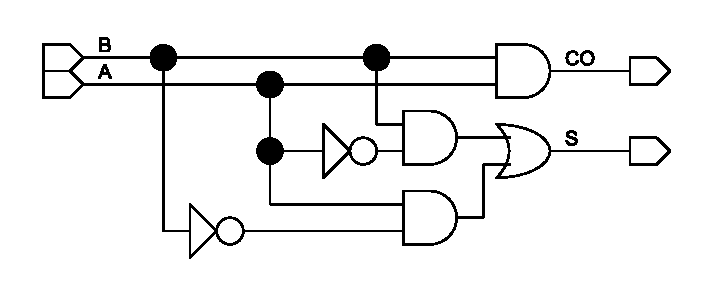
\includegraphics[width=\hsize]{human_ha.eps}
   \caption{a way to encode schematic for input vector of neural network}
   \label{fig:human_ha}
  \end{minipage}
 \end{center}
\end{figure}

Figure \ref{fig:conventional} shows a schematic of a half added
composed only of and, or and not gates, automatically generated
from a netlist by a CAD software.
Figure \ref{fig:human_ha} shows a logically identical one drawn by a human.
It has less curve and cross points than one generated by a CAD.
In this work, a way to revise schematics from one like
figure \ref{fig:conventional} to the other like figure \ref{fig:human_ha}
is shown.

\begin{figure}[tb]
 \begin{center}
  \begin{minipage}{\hsize}
   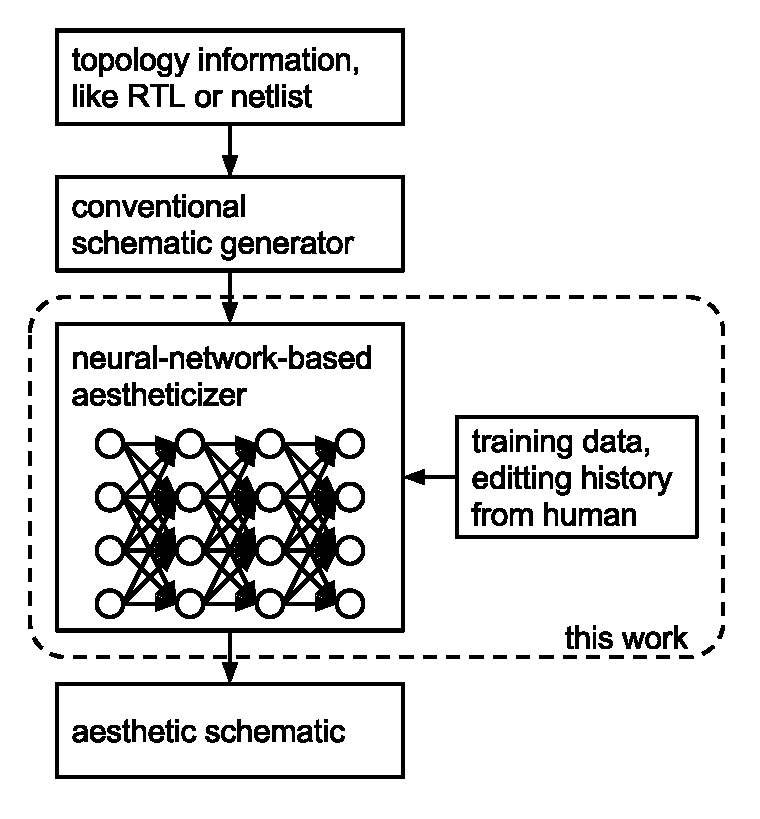
\includegraphics[width=\hsize]{flow.eps}
   \caption{a flow to obtain an aesthetic schematic}
   \label{fig:flow}
  \end{minipage}
 \end{center}
\end{figure}

Figure {\ref{fig:flow}} shows a concept how to obtain an aesthetic schamatic.
It has a neural network which learns pairs of schematic and editting command
issued by a human.
Whichever the schematic is given by a conventional schematic generator
or other human,
the trained neural network update the schematic.

\begin{figure}[tb]
 \begin{center}
  \begin{minipage}{\hsize}
   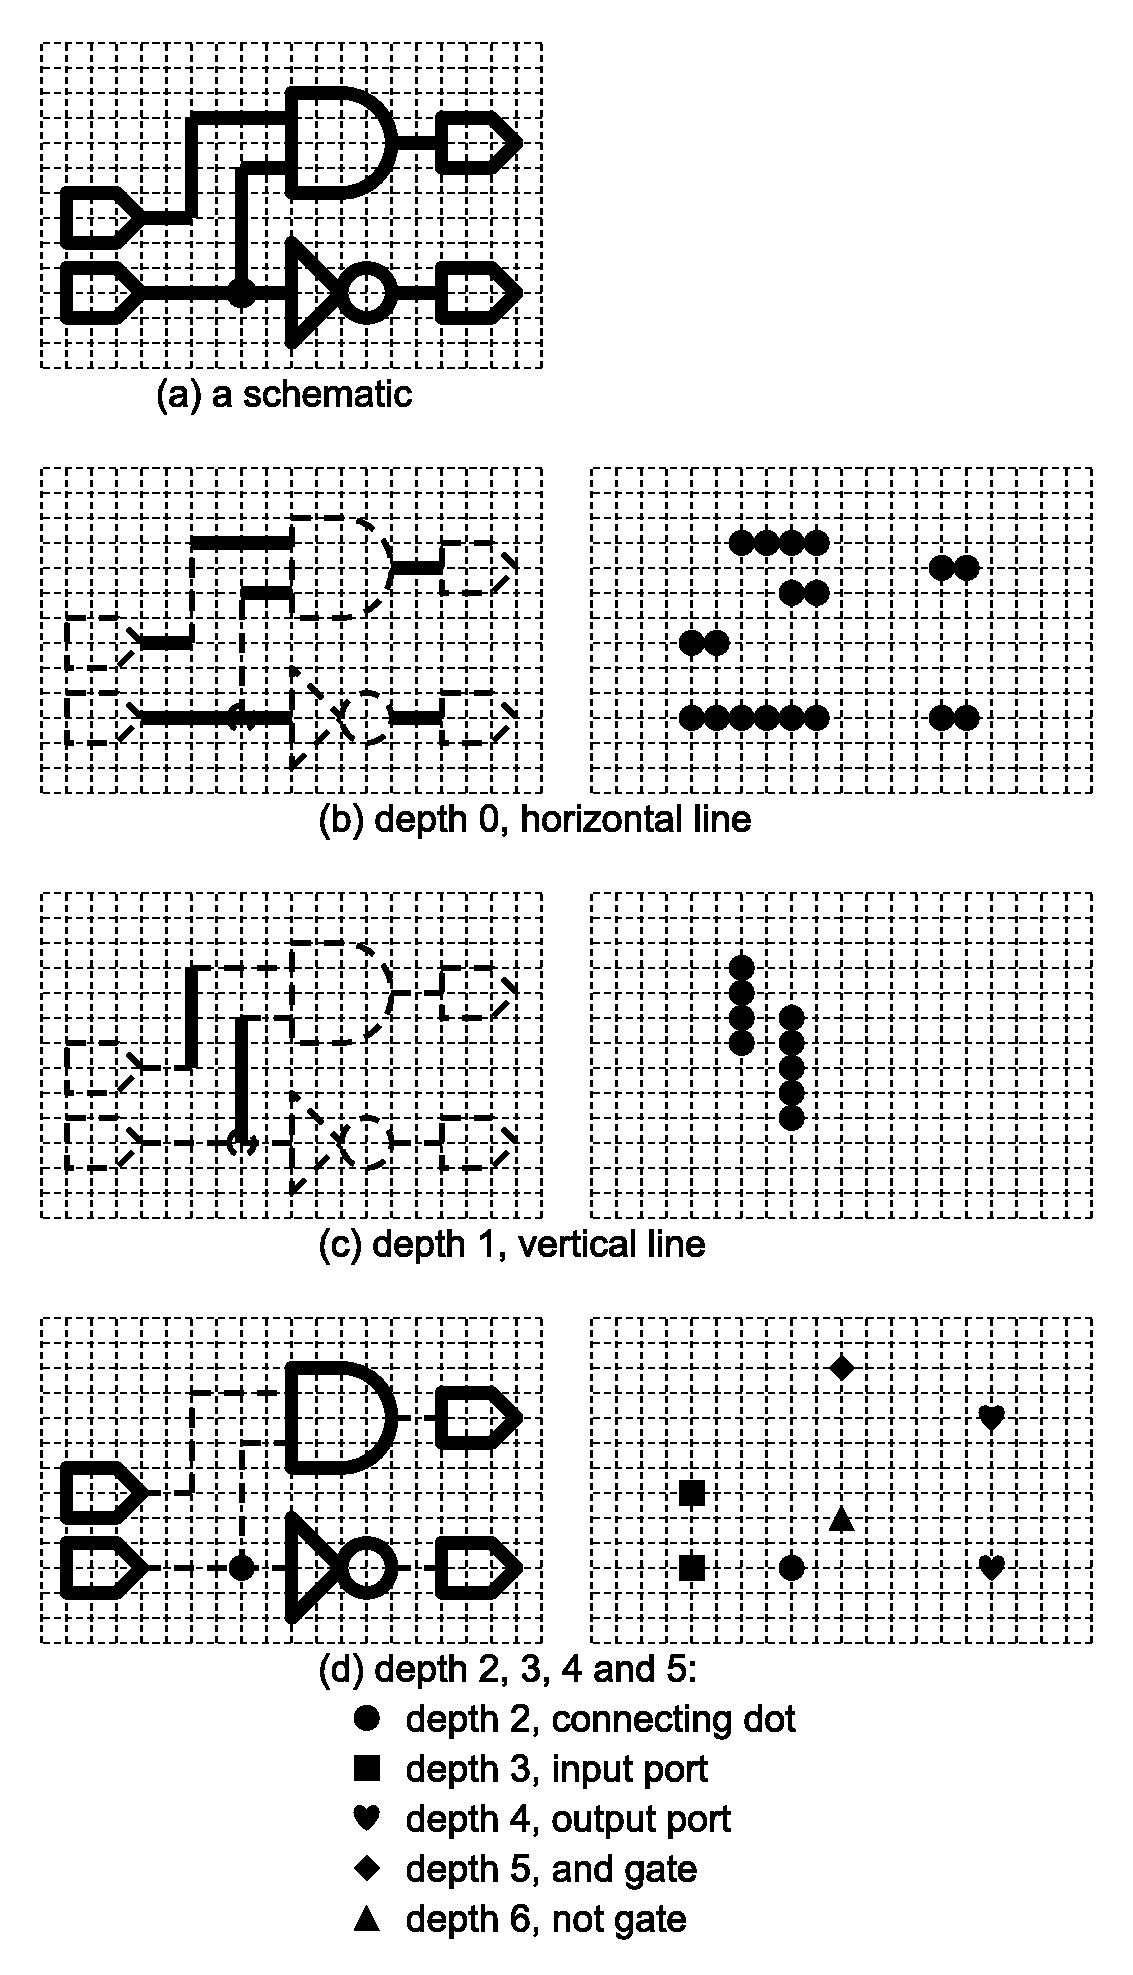
\includegraphics[width=\hsize]{input_encode_03.eps}
   \caption{a way to encode schematic for input vector of neural network}
   \label{fig:input_encode}
  \end{minipage}
 \end{center}
\end{figure}

\begin{figure}[tb]
 \begin{center}
  \begin{minipage}{\hsize}
   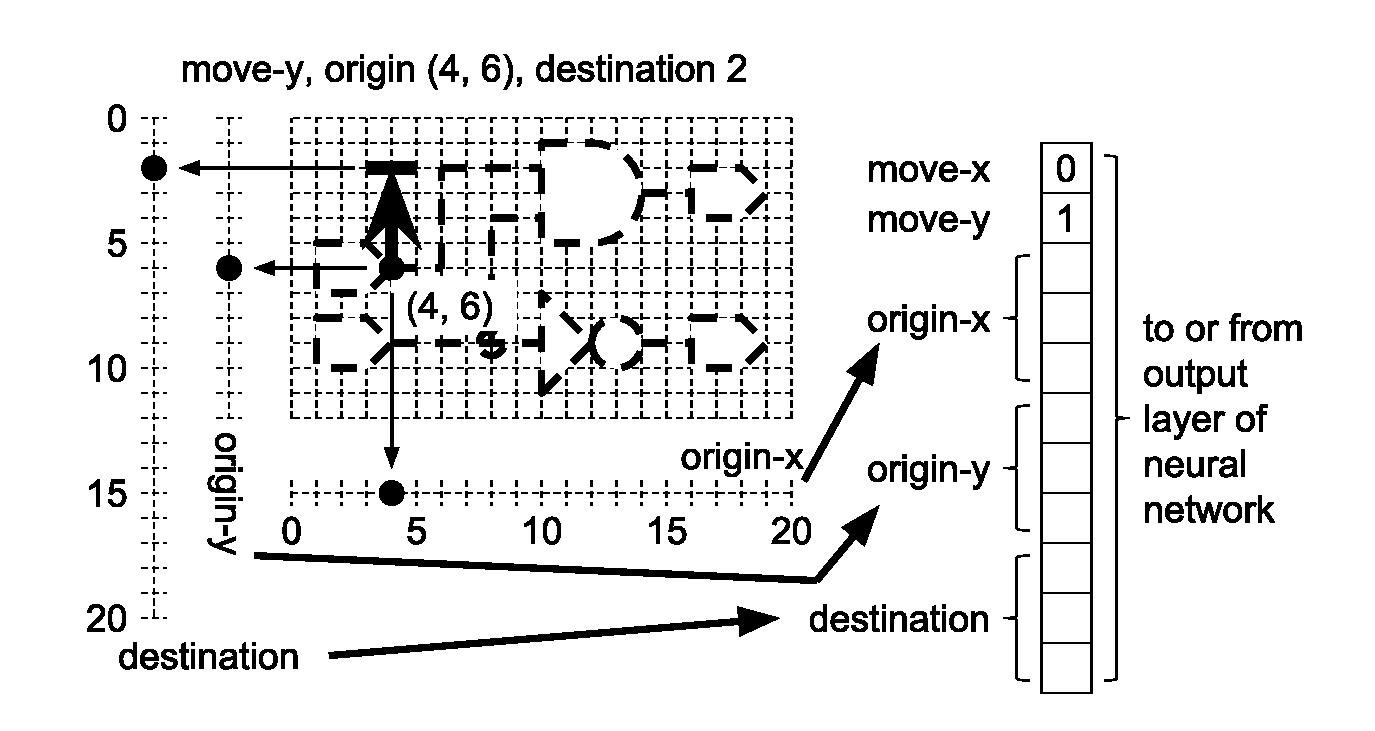
\includegraphics[width=\hsize]{output_encode_02.eps}
   \caption{a way to encode schematic for output vector of neural network}
   \label{fig:output_encode}
  \end{minipage}
 \end{center}
\end{figure}

To feed schematics and editing command to neural network,
they are necessary to be encoded into vectors composed of real numbers.
Figure \ref{fig:input_encode} shows the way to encode schematic.
Figure \ref{fig:input_encode} (a) shows a logic schematic composed of
inputs ports, output ports, an and-gate, a not-gate,
horizontal nets, vertical nets, and a connecting point.
Figure \ref{fig:input_encode} (b) picks up horizontal nets appearing
in Figure \ref{fig:input_encode} (a), and they are mapped to depth 0.
Depth 0 composed of a 2-dimensional matrix which size is the same
as given schematic.
In the right side of figure \ref{fig:input_encode},
dots are located at coordinates where horizontal nets appear.
Points with dots corresponds to a value of 1.0, ones without dots
corrensponds to a value of 0.0.
As shown in figure \ref{fig:input_encode} (c),
vertical nets are mapped to depth 1.
As well, connecting dots, input ports, output ports, and-gates and not-gates
are mapped to depth 2, 3, 4, 5 and 6, respectively.
Input vectors are finally obtained by flattening the multi-layer of matrices.

Figure \ref{fig:output_encode} shows a way to encode editing commands
for output vector of the neural network.
A command `move-y, origin (4, 6), destination 2' is shown in the figure
as an example, which means to vertically move a object at the point (4, 6)
to y-coordinate of 2.
The more general explanation of editing commands follow.
Editing command consist of three elements.
The first element is a type of command.
Only 2 kinds of commands are used in this paper,
which are move-x and move-y,
although the other commands could be introduced as long as
the command would not change the semantics of the schematic.
Move-x means to move a object horizontally.
Move-y means to move one vertically.
The second element is a 2-element vector, meaning origin of the command.
The vector consists of x and y coordinates of the origin.
The third element is destination.
The destination means x-coordinate when the type of command
is move-x, in this work.
It becomes y-coordinates when the command if move-y.
Move-x is encoded to the vector $[1.0, 0.0]$, 
while move-y is encoded to the vector $[0.0, 0.1]$. 
The x coordinate of origin is encoded to so-called one-hot vector,
which is
$[1.0, 0.0, 0.0, 0.0, \cdots]$ for 0,
$[0.0, 1.0, 0.0, 0.0, \cdots]$ for 1, 
$[0.0, 0.0, 1.0, 0.0, \cdots]$ for 2,
and so on. The length of one-hot vector is chosen as the width of
the schematic.
The y coordinate is also encoded to one-hot vector which length is
height of the schematic.
As well, destination is one-hot vector which length is
maximum value of width and height of the schematic.
Output vector of the neural network is eventually obtained
by concatenating those 4 one-hot vectors.

\begin{figure}[tb]
 \begin{center}
  \begin{minipage}{\hsize}
   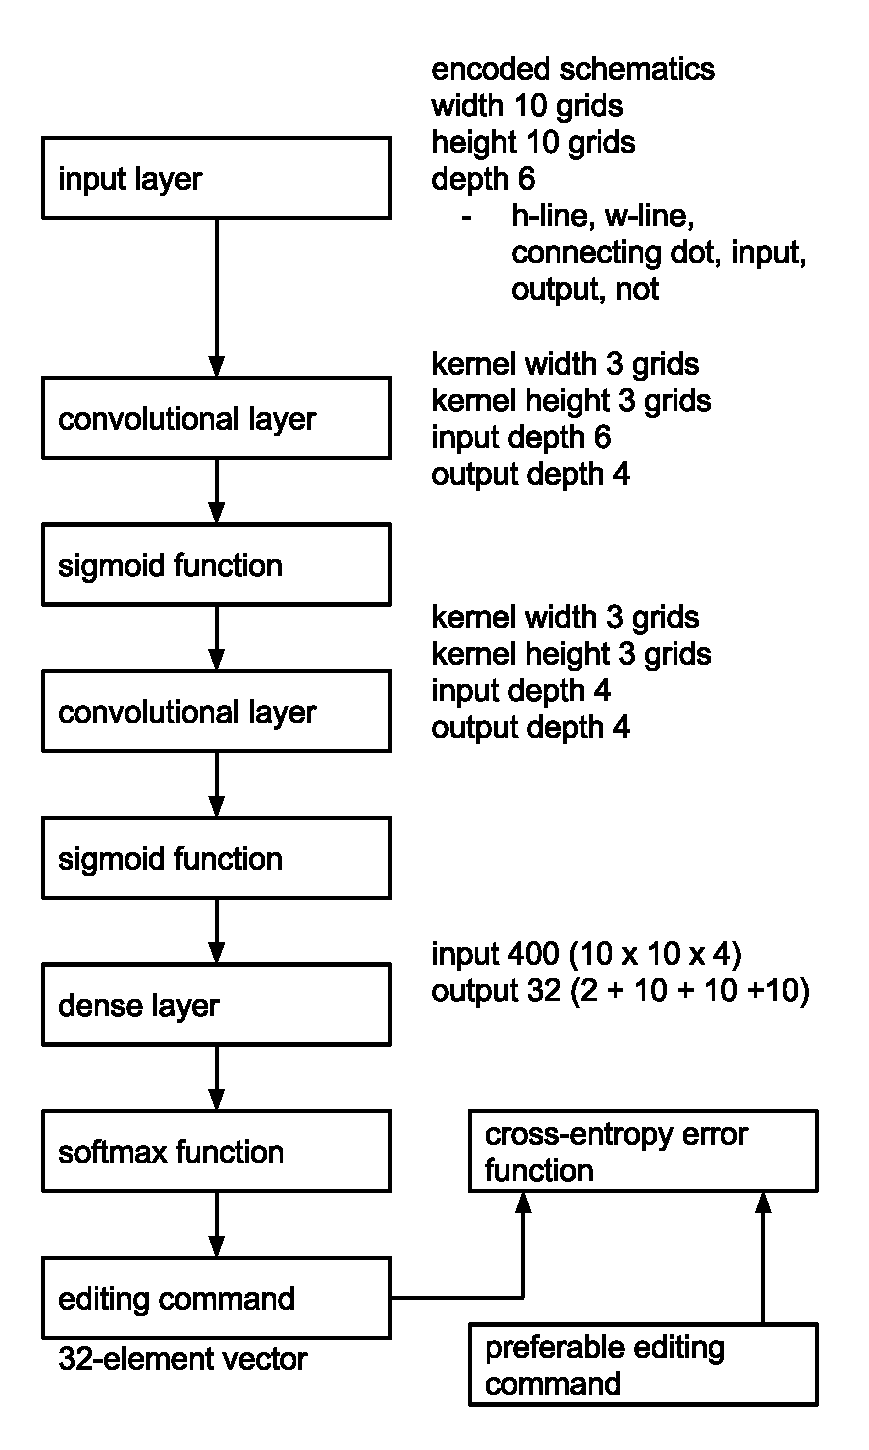
\includegraphics[width=\hsize]{layers.eps}
   \caption{a way to encode schematic for output vector of neural network}
   \label{fig:layers}
  \end{minipage}
 \end{center}
\end{figure}

\begin{figure}[tb]
 \begin{center}
  \begin{minipage}{\hsize}
   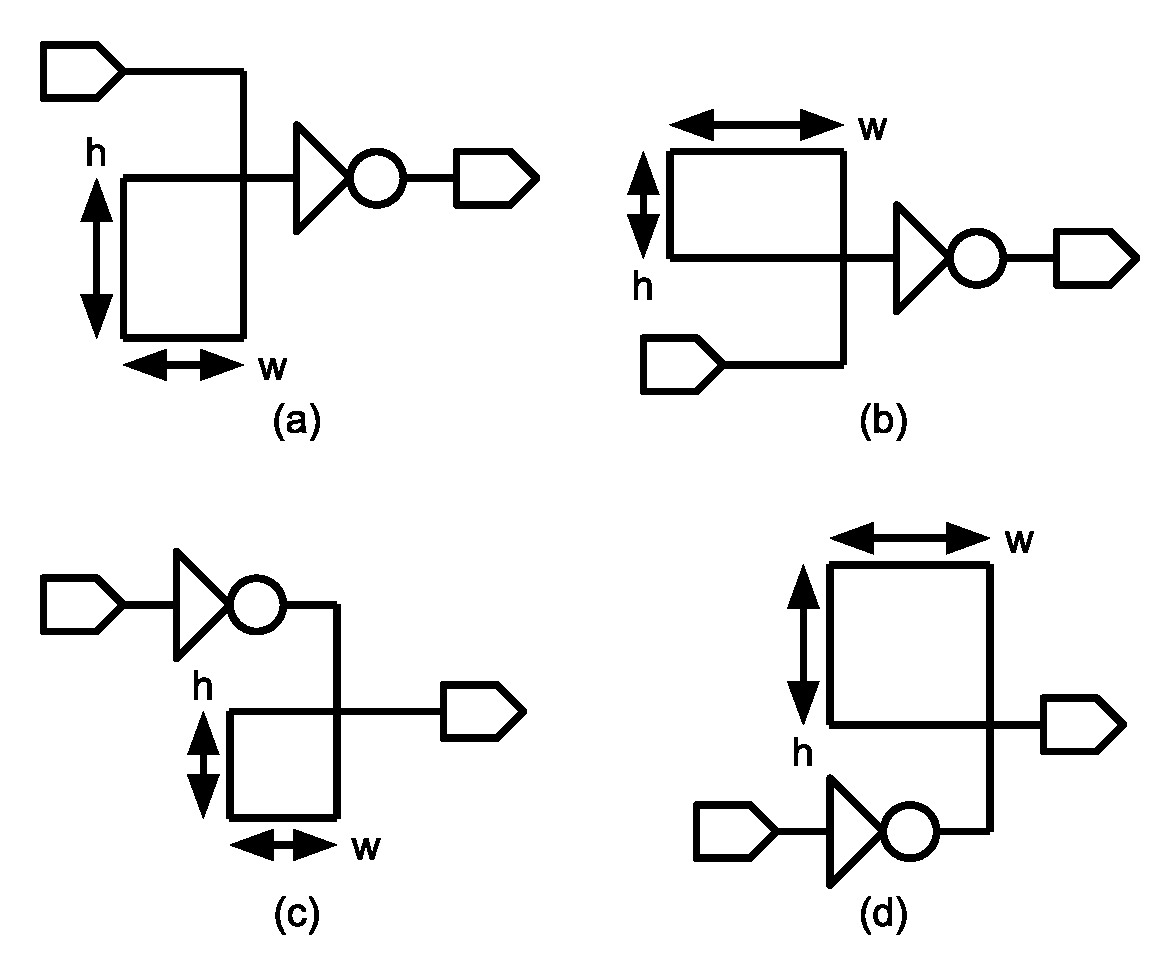
\includegraphics[width=\hsize]{fig/training_data_01.eps}
   \caption{training data}
   \label{fig:training_data}
  \end{minipage}
 \end{center}
\end{figure}

\begin{figure}[tb]
 \begin{center}
  \begin{minipage}{\hsize}
   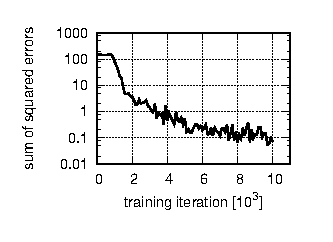
\includegraphics[width=\hsize]{fig/errors.eps}
   \caption{convergence of error}
   \label{fig:errors}
  \end{minipage}
 \end{center}
\end{figure}

\begin{figure}[tb]
 \begin{center}
  \begin{minipage}{\hsize}
   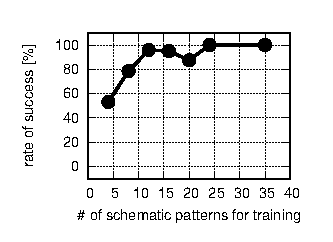
\includegraphics[width=\hsize]{fig/test_data.eps}
   \caption{rate of success of revising the schematics}
   \label{fig:test_data}
  \end{minipage}
 \end{center}
\end{figure}

\section{Summary and Conclusions}

This template can be downloaded through the ASP-DAC 2018 web site
(http://www.aspdac.com/). If you have any problem, please contact ASP-DAC
2018 publication chair (jlee@unist.ac.kr).

%this is how to do an unnumbered subsection 
\section*{\sc Acknowledgements}
This article was written by referring to {\em ``Author's guide --
Preparation of Papers in Two-Column Format for VLSI Symposia on
Technology and Circuits''}, the {\em ``Preparation of Papers in
Two-Column Format for the Proceedings of the 32nd ACM/IEEE Design
Automation Conference''} written by Ann Burgmeyer, IEEE and {\em ``the
template for producing IEEE-format articles using \LaTeX''}, written by
Matthew Ward, Worcester Polytechnic Institute.

\begin{thebibliography}{9}
\footnotesize
\bibitem{key}
I. M. Author,
``Some related article I wrote,''
{\em Some Fine Journal}, vol. 17, pp. 1--100, 1987.

\bibitem{baz}
A. N. Expert,
{\em A Book He Wrote,}
His Publisher, 1989.

\bibitem{unpub}
M. Smith,
``Title of paper optional here,''
unpublished.

\bibitem{inpress}
K. Rose,
``Title of paper with only first word capitalized,''	% bug fixed by M. Imai
in press.

\bibitem{trans}
T. Murayama,
``Title of paper published in translation journals,''	% bug fixed by M. Imai
{\em Some English Journal}, vol. 17, pp. 1--100, 1995.	% bug fixed by M. Imai
({\em Original Foreign Journal, vol. 1, pp. 100-200, 1993}.)	% ditto

\end{thebibliography}
\end{document}
